
\documentclass{standalone}

\usepackage[OT1]{fontenc}
\renewcommand*\familydefault{\sfdefault}
\usepackage{helvet,sfmath}
\usepackage{siunitx}

\usepackage{tikz}
\usetikzlibrary{arrows,calc,patterns}
% \usetikzlibrary{intersections, calc, arrows.meta}
\usepackage{tikz,tkz-euclide}
\usepackage{amsmath}
\usepackage[utf8]{vietnam}
\usepackage[T5]{fontenc}

\begin{document}
\tikzset{every picture/.style={line width=0.75pt}} %set default line width to 0.75pt        

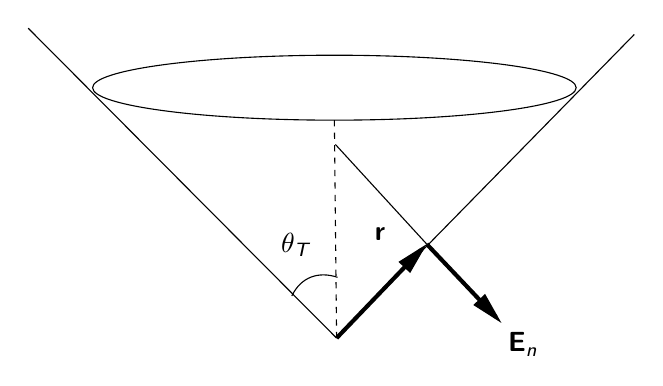
\begin{tikzpicture}[x=0.75pt,y=0.75pt,yscale=-1,xscale=1]
%uncomment if require: \path (0,300); %set diagram left start at 0, and has height of 300

%Straight Lines [id:da477806425534132] 
\draw    (141.43,30.71) -- (290,180) ;
%Straight Lines [id:da3193423659756527] 
\draw    (433.43,33.71) -- (290,180) ;
%Straight Lines [id:da25585832494924077] 
\draw  [dash pattern={on 2.25pt off 2.25pt on 2.25pt off 2.25pt}]  (288.93,75) -- (290,180) ;
%Shape: Ellipse [id:dp020111536491030813] 
\draw   (172.43,59.36) .. controls (172.43,50.72) and (224.59,43.71) .. (288.93,43.71) .. controls (353.27,43.71) and (405.43,50.72) .. (405.43,59.36) .. controls (405.43,68) and (353.27,75) .. (288.93,75) .. controls (224.59,75) and (172.43,68) .. (172.43,59.36) -- cycle ;
%Curve Lines [id:da7763609453534744] 
\draw    (268.43,159.71) .. controls (272.86,150.43) and (281.43,147.71) .. (290.43,150.71) ;
%Straight Lines [id:da4333818805346543] 
\draw [line width=1.5]    (290,180) -- (330.66,137.6) ;
\draw [shift={(333.43,134.71)}, rotate = 133.8] [fill={rgb, 255:red, 0; green, 0; blue, 0 }  ][line width=0.08]  [draw opacity=0] (15.6,-3.9) -- (0,0) -- (15.6,3.9) -- cycle    ;
%Straight Lines [id:da9660817509501911] 
\draw [line width=1.5]    (366.68,169.81) -- (333.43,134.71) ;
\draw [shift={(369.43,172.71)}, rotate = 226.55] [fill={rgb, 255:red, 0; green, 0; blue, 0 }  ][line width=0.08]  [draw opacity=0] (15.6,-3.9) -- (0,0) -- (15.6,3.9) -- cycle    ;
%Straight Lines [id:da5878407626357527] 
\draw    (289.43,86.71) -- (333.43,134.71) ;

% Text Node
\draw (262,128.4) node [anchor=north west][inner sep=0.75pt]    {$\theta _{T}$};
% Text Node
\draw (307.21,125.76) node [anchor=north west][inner sep=0.75pt]    {$\mathbf{r}$};
% Text Node
\draw (371.43,176.11) node [anchor=north west][inner sep=0.75pt]    {$\mathbf{E}_n$};


\end{tikzpicture}

\end{document}